\documentclass{beamer}
\usepackage[utf8]{inputenc}
\usepackage[T1]{fontenc}
\usepackage{url}
\usepackage{hyperref}
\usepackage{xcolor}
\usepackage[french]{babel}
\usepackage{appendixnumberbeamer}
\usetheme[sectionpage=none,
          subsectionpage=progressbar,
          numbering=fraction,
          progressbar=none,
          background=light]{metropolis}

\title{Introduction à Python pour la Data Science}
\subtitle{Cours de statistiques descriptives --- TD}
\date{2019}
\author{\textsc{Florent Forest}\vspace{0.2cm}\\

\includegraphics[height=0.35cm]{./rc/e-mail-envelope-blue}\;\scriptsize{\href{mailto:forest@lipn.univ-paris13.fr}{forest@lipn.univ-paris13.fr}}\\

\includegraphics[height=0.35cm]{./rc/grid-world-blue}\;\scriptsize{\href{http://florentfo.rest}{http://florentfo.rest}}\\

\includegraphics[height=0.35cm]{./rc/github-logo-blue}\;\scriptsize{\href{https://github.com/FlorentF9}{FlorentF9}}\\
}
\institute{\vfill\hfill

\includegraphics[height=1.0cm]{./rc/up13_logo}
\hspace{0.1cm}

\includegraphics[height=1.0cm]{./rc/supgalilee_logo}}

\begin{document}

  \maketitle

  \begin{frame}{Démarrage}

    \begin{center}
      $\blacktriangleright$ \href{https://github.com/FlorentF9/SupGalilee-tdstats}{github.com/FlorentF9/SupGalilee-tdstats}
    \end{center}

    \vspace{1cm}

    \metroset{block=fill}
    \begin{block}{Prérequis}
      \begin{itemize}
        \item[>] \texttt{git} : Système de gestion de versions (VCS = version control system)
        \item[>] \texttt{docker} : Gestionnaire de conteneurs d'applications
      \end{itemize} 
    \end{block}
  
  \end{frame}

  \begin{frame}{git}

    \begin{center}
      
\includegraphics[height=1.5cm]{./rc/git.png}
    \end{center}

    \texttt{\$ git --version}

    \begin{block}{Linux}
      \texttt{sudo apt install git}
    \end{block}

    \begin{block}{Autres OS}
      \href{https://git-scm.com/downloads}{https://git-scm.com/downloads}
    \end{block}
    
  \end{frame}

  \begin{frame}{docker}

    \begin{center}
      
\includegraphics[height=2cm]{./rc/docker-logo.png}
    \end{center}

    \texttt{\$ docker --version}

    \begin{block}{Linux}
      \texttt{sudo apt install docker.io} 
    \end{block}

    \begin{block}{Autres OS}
      \href{https://docs.docker.com/docker-for-windows/install/}{https://docs.docker.com/docker-for-windows/install/}, \href{https://docs.docker.com/docker-for-mac/install/}{https://docs.docker.com/docker-for-mac/install/}
    \end{block}
    
  \end{frame}

  \begin{frame}{docker}
    
    \metroset{block=fill}
    \begin{block}{Pourquoi utiliser docker ?}
      \begin{itemize}
        \item[>] Applications \textbf{isolées} du reste du système
        \item[>] Environnements \textbf{prêts-à-l'emploi} et \textbf{identiques} pour chaque étudiant
      \end{itemize} 
    \end{block}

    \begin{center}
      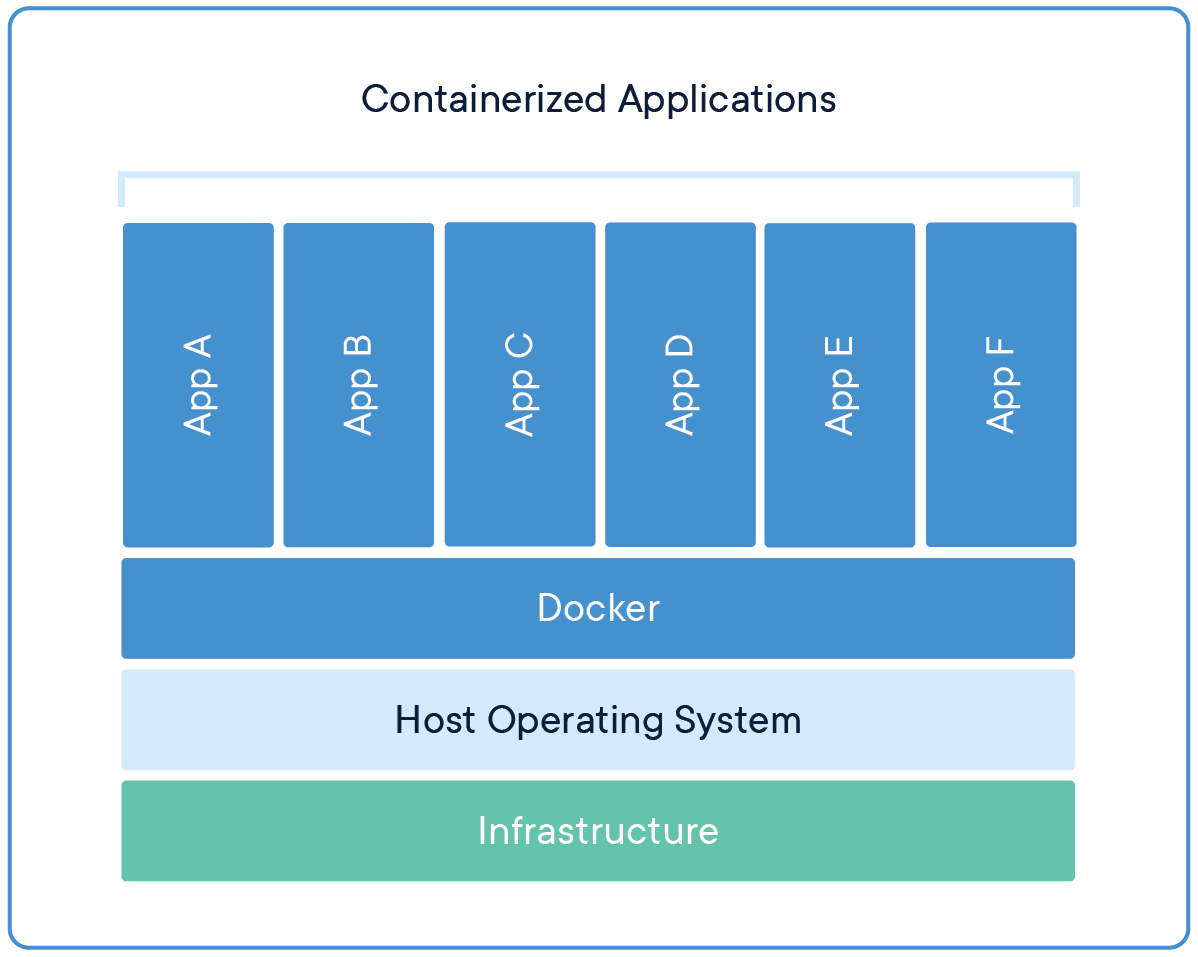
\includegraphics[width=5.5cm]{./rc/containers.png}
      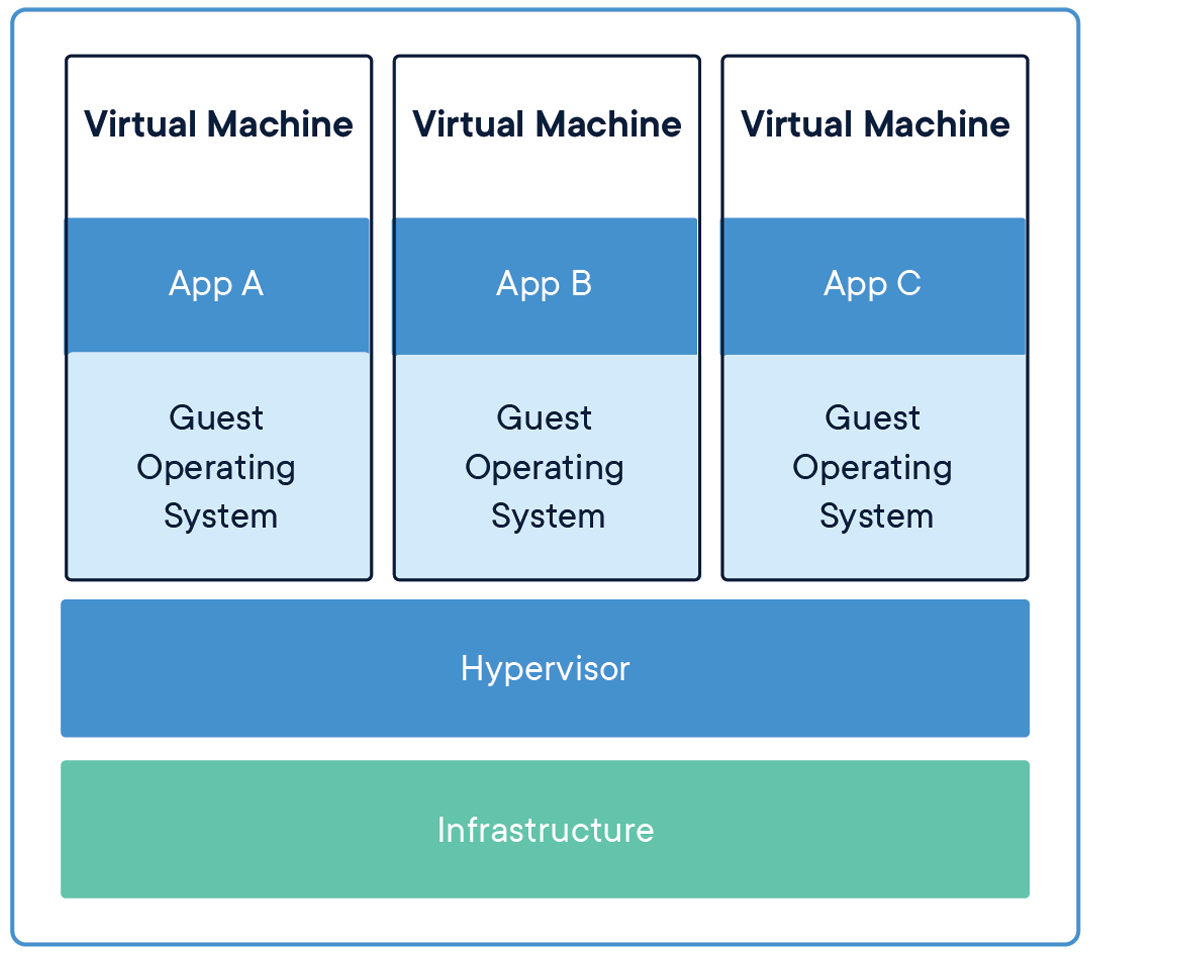
\includegraphics[width=5.5cm]{./rc/vms.png}
    \end{center}

  \end{frame}

  \begin{frame}{C'est parti !}

    \begin{center}
      $\blacktriangleright$ \href{https://github.com/FlorentF9/SupGalilee-tdstats}{github.com/FlorentF9/SupGalilee-tdstats}
    \end{center}

    \begin{enumerate}
      \item Clonez le dépôt github et placez-vous à l'intérieur.\\
      \texttt{\$ git clone git@github.com:FlorentF9/SupGalilee-tdstats.git}\\
      \texttt{\$ cd SupGalilee-tdstats}
      \item Construisez l'image docker.\\
      \texttt{\$ docker build . -t tdstats}
      \item Démarrez un conteneur en associant un port et un volume.\\
      \texttt{\$ docker run -it --rm -p 9999:9999 -v `pwd`/td:/td tdstats}
      \item Cliquez sur le lien \texttt{http://127.0.0.1:9999/?token=XXX}. L'environnement Jupyter Lab devrait s'ouvrir dans votre navigateur !
    \end{enumerate}

  \end{frame}

  \begin{frame}{C'est parti !}
    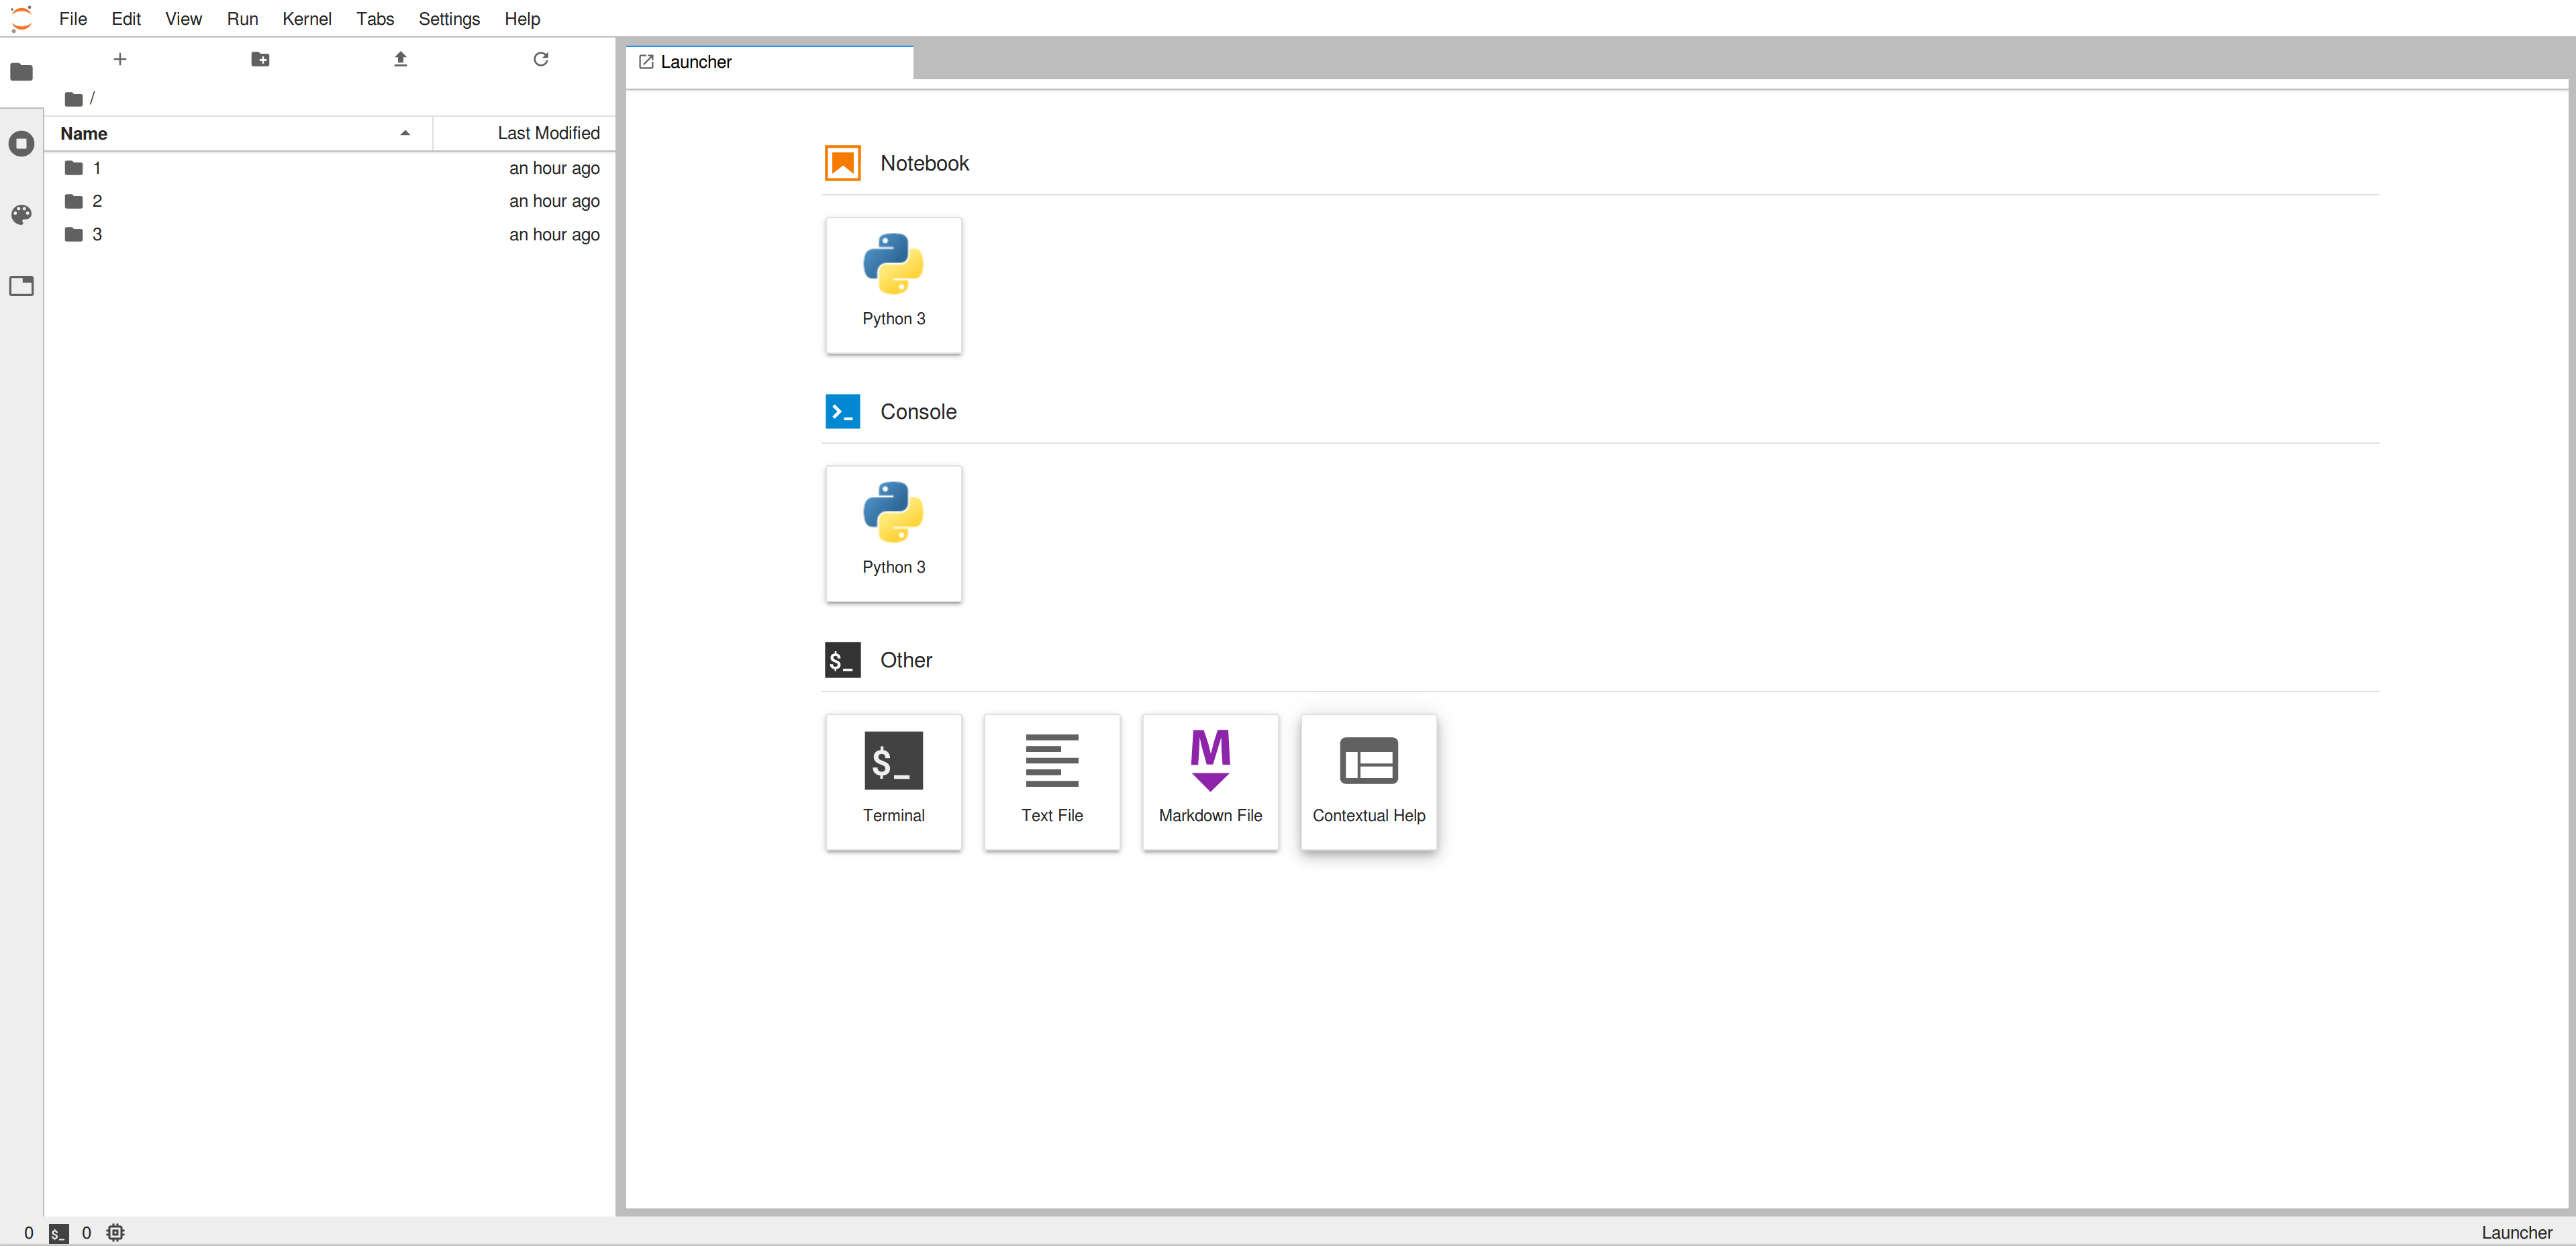
\includegraphics[width=11cm]{./rc/jupyter-lab.png}
  \end{frame}


\end{document}
